The selection of an appropriate microcontroller was a critical aspect of the hardware design for this project. Given the project’s constraints and the need to utilize available components, it was necessary to choose a microcontroller based on readily accessible development boards. After evaluating several options, the ESP32 was identified as the most suitable choice due to its versatile features and broad compatibility with the project’s requirements.\\
The ESP32 microcontroller is a highly versatile and capable device that offers a broad range of features, making it ideal for this project. At its core, the ESP32 incorporates a dual-core, 32-bit Tensilica LX6 microcontroller, based on the Harvard architecture. This architecture separates data and instruction memory, enhancing processing efficiency. The CPU speed is adjustable, ranging from \num{160}~\si{\mega\hertz} to \num{240}~\si{\mega\hertz}, allowing the system to optimize for either performance or energy consumption depending on the operational requirements~\cite{Kareem.2021}. It offers several advantages over other similarly priced microprocessor. Its very low power consumption is particularly beneficial in battery-powered systems like this remote controlled vehicle, extending operational time while minimizing energy drain. Additionally, the ESP32 boasts a high level of integration, including a built-in antenna and step-down converter, simplifying the overall hardware design and reducing the need for additional components~\cite{espressif.07.09.2024}.\\
The ESP32 Dev Kit C is a widely used development board, designed for easy prototyping with the ESP32 microcontroller, it can be seen in fig.~\ref{fig:microprocessor_esp32}. The key components of the board are marked as follows:
\begin{enumerate}
	\item \textbf{Micro USB connector}: Used for powering the board and programming the ESP32 via a USB connection.
	\item \textbf{AMS1117 Voltage regulator}: Ensures the board operates at the required \num{3.3}~\si{\volt} by stepping down input voltage from the Vin pin or the USB connection.
	\item \textbf{CP2102 USB to UART bridge}: Facilitates communication between the USB port and the ESP32, enabling data transfer and debugging.
	\item \textbf{ESP32-WROOM-32 module}: The heart of the board, containing the ESP32 microcontroller.
	\item \textbf{Antenna}: Built-in antenna for wireless communication.
\end{enumerate}
Other notable connections include:
\begin{itemize}
	\item \textbf{GND}: Ground connection used as the negative voltage reference.
	\item \textbf{3V3}: Provides \num{3.3}~\si{\volt} output or requires exactly \num{3.3}~\si{\volt} of input supply voltage for stable operation.
	\item \textbf{Vin}: Can accept a wide input voltage range from \num{4.4}~\si{\volt} to \num{12}~\si{\volt}~\cite{amicu.}, regulated down to \num{3.3}~\si{\volt} internally.
\end{itemize}

\begin{figure}[h]
	\centering
	\captionsetup{justification=centering}
	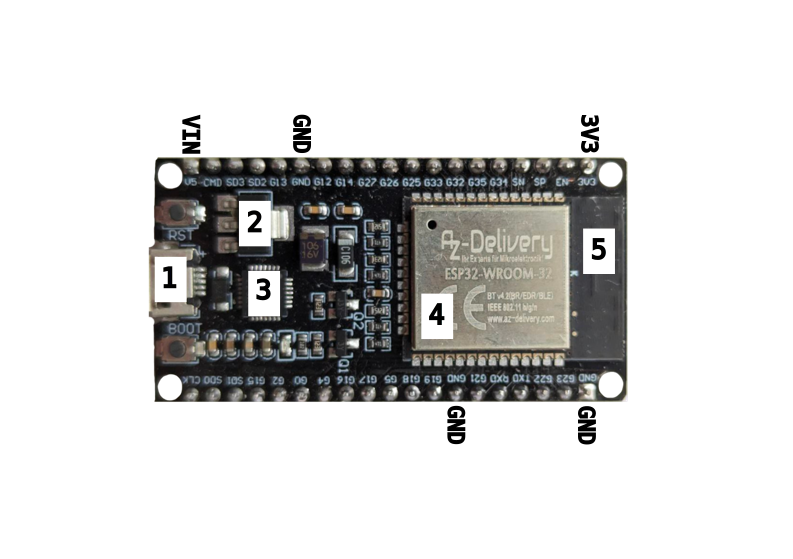
\includegraphics[width=0.6\linewidth]{esp32_board.pdf}
	\caption{ESP32 Dev Kit C Board}
	\label{fig:microprocessor_esp32}
\end{figure}

The ESP32 also boasts an extensive range of input and output (I/O) options. It has 36 \ac{gpio} pins, 18 of which can be used as \ac{adc} inputs, allowing the microcontroller to read sensor data and other analog signals. Furthermore, the ESP32 is equipped with two dedicated \ac{dac} pins, which can generate true analog outputs, a feature that is particularly useful in applications where precise control over analog signals is required. Almost all output-capable pins can also produce \ac{pwm} signals, which are integral to this project for controlling motor speed and direction~\cite{Kareem.2021}.\\
In terms of memory, the ESP32 features both on-chip (internal) and onboard (external) memory. The internal memory is composed of 448 KB of ROM, which is responsible for booting and core functions, and 520 KB of SRAM used for data storage and instructions during runtime. Additionally, the ESP32 supports up to 16 MB of external ISP flash RAM, which can be used to store larger programs or data sets that exceed the capacity of the internal memory~\cite{Kareem.2021}.
One of the ESP32’s most significant features is its built-in communication capabilities. For wireless communication, it supports WiFi with full 802.11 b/g/n/e/i standards. This allows the ESP32 to function as both a client, connecting to a router, and as an access point, creating its own wireless network. This versatility is beneficial for remotely controlling the vehicle via \ac{udp} packets over WiFi. The Bluetooth module supports v4.2 BR/EDR and \ac{ble} standards, with data transfer speeds of up to 4.0~Mbps, making it possible to control the vehicle with Bluetooth devices, such as a \ac{ps4} controller~\cite{Kareem.2021}.\\
In addition to its wireless communication, the ESP32 supports several wired communication protocols, including UART, I2C, ISP, CAN, and I2S. These protocols allow the microcontroller to communicate with a variety of peripheral devices, such as sensors, motor drivers, and other controllers, providing flexibility in system design and integration~\cite{Kareem.2021}.\\
The ESP32 can be programmed using two main frameworks. The first, ESP-IDF, is the official development framework provided by Espressif Systems. It offers low-level access to the hardware and allows developers to take full advantage of the ESP32's dual-core architecture. However, due to its complexity, it is more suited for advanced projects requiring intricate customization. The second framework is the Arduino IDE, which simplifies development by abstracting some of the low-level details~\cite{Kareem.2021}. Although it offers less flexibility in core management compared to ESP-IDF, the Arduino framework provides sufficient functionality for this project and is widely supported with extensive libraries and an open-source community. Given the project's requirements and the ease of development, the Arduino framework was chosen for this application.